% vim:tw=70
\documentclass[ignorenonframetext]{beamer}
%\documentclass{article}
%\usepackage{beamerarticle}

\RequirePackage{fix-cm}

\mode<presentation>{\usetheme{Darmstadt}}
%\usetheme{default}
%\usetheme{Singapore}
%\usetheme{Dresden}
%\usetheme{Luebeck}
%\usetheme{Antibes}
%\usetheme{Malmoe}

\mode<presentation>{\usepackage{latex/elephantbird}}
%\usecolortheme{beetle}
%\usecolortheme{seahorse}
%\usecolortheme{dolphin}
%\usecolortheme{whale}
%\usecolortheme{fly}

\usepackage{rotating}
\usepackage[utf8]{inputenc}

\usepackage{amsmath,amssymb,amsfonts,textcomp}
\usepackage{amsthm}
\usepackage{array}
\usepackage[english]{babel}
\usepackage[T1]{fontenc}
\usepackage{graphicx}
%\usepackage{theorem}
\usepackage{enumerate}
\usepackage{color}
\usepackage{framed}
\usepackage{url}
\usepackage{hyperref}
\usefonttheme{professionalfonts}
%\usefonttheme{serif}

\def\nq{\hspace{-1em}}
\def\look{\(\uparrow\)}
\def\ignore#1{}
\def\deltabar{{\delta\!\!\!^{-}}}
\def\qed{\sqcap\!\!\!\!\sqcup}
\def\odt{{\textstyle{1\over 2}}}
\def\odf{{\textstyle{1\over 4}}}
\def\odA{{\textstyle{1\over A}}}
\def\hbar{h\!\!\!\!^{-}\,}
\def\dbar{d\!\!^{-}\!}
\def\eps{\varepsilon}
\def\beq{\begin{equation}}
\def\eeq{\end{equation}}
\def\beqn{\begin{displaymath}}
\def\eeqn{\end{displaymath}}
\def\bqa{\begin{equation}\begin{array}{c}}
\def\eqa{\end{array}\end{equation}}
\def\bqan{\begin{displaymath}\begin{array}{c}}
\def\eqan{\end{array}\end{displaymath}}
\def\pb{\underline}                       % probability notation
\def\pb#1{\underline{#1}}                 % probability notation
\def\blank{{\,_\sqcup\,}}                 % blank position
\def\maxarg{\mathop{\rm maxarg}}          % maxarg
\def\minarg{\mathop{\rm minarg}}          % minarg
\def\hh#1{{\dot{#1}}}                     % historic I/O
\def\best{*}                              % or {best}
\def\vec#1{{\bf #1}}
\def\length{{l}}

\title{Reinforcement Learning}
\author{Josh Bryan}
\institute{University of Illinois at Chicago, MCS 548}
\date{\today}

\newcommand{\argmax}{\operatornamewithlimits{argmax}}



\begin{document}

\maketitle

\section{Introduction}
\mode<presentation>{
\subsection{Title}
\begin{frame}
	\titlepage
\end{frame}
\subsection{Contents}
\begin{frame}[allowframebreaks]
	\tableofcontents
\end{frame}
}


\subsection{Reinforcement Learning Overview}

	Reinforcement Learning is an area of AI at the boundary between machine
	learning and decision theory that also incorporates ideas from
	psychology.  The basic learning task is to learn an agent function,
	a function mapping a sequence of observations to an action, by
	actively participating in and exploring an environment.  The
	fundamental idea is that for every action the agent receives some form of
	reward signal.  That signal is the agents indication of success, and
	its task is to maximize the expectation of average or discounted sum
	of rewards.  For the most part this presentation will follow the
	the exposition given in Chapter 13 of \cite{mitchell_machine_1997},
	however ideas will be borrowed from
	\cite{kaelbling_reinforcement_1996} and
	\cite{russell_artificial_2010} as well.  

\begin{frame}
	\frametitle{What is Reinforcement Learning?}
	\begin{block}{}
		Reinforcement learning takes psychology, decision theory, and
		learning theory to answery ``How should an agent learn to act?''
	\end{block}
	\begin{itemize}
		\item Classical Conditioning (Pavlov's Dog)
		\item Utility Theory
		\item (Partially Observable) Markov Decision Processes
		\item Learns an ``Agent Function''
	\end{itemize}
\end{frame}

\begin{frame}
	\frametitle{Agent Function}
	\begin{itemize}
		\item $O$ is a set of observation symbols.
		\item $A$ is a set of actions.
	\end{itemize}
	\begin{block}{}
		\begin{center}
			$f: O^* \rightarrow A $
		\end{center}
	\end{block}
\end{frame}

\begin{frame}
	\frametitle{Uses}
	\begin{itemize}
		\item Game playing (e.g. back gammon)
		\item Learning tasks with delayed feedback
		\item Elevator Control
		\item Robotic Control (e.g. stick balancing, car driving)
		\item Simulation Based Approximation Methods (similar to
			ficticious play)
		\item Telecomunication (e.g. learning optimal
			routing)
	\end{itemize}
\end{frame}

\section{Markov Decision Processes}

\subsection{Model Introduction}

A Markov Decision Process describes a system in which an agent exists
in a state $s_t \in S$ at time $t$.  In each state, the agent must choose
an action $a_t \in A$.  After choosing an action, the agent will
transition from $s_t$ to $s_{t+1}$ according to a probability
distribution $T(s_t, a_t, s_{t+1}) = P(s_{t+1} | s_t, a_t)$.

\begin{frame}
	\frametitle{What is an MDP?}
	\begin{block}{Definition: Markov Decision Process}
		An MDP is a tuple $\langle S, A, T, R \rangle$ where:
		\begin{description}
			\item[S] is a set of states.
			\item[A] is a set of actions.
			\item[T] is a transition function. 
				\[ T: S\times A\times S \rightarrow [0,1] \]
			\item[R] is a reward function. 
				\[ R: S\times A \rightarrow \mathbb{R} \] 
		\end{description}
	\end{block}
\end{frame}

\begin{frame}
	\frametitle{Simple Example}
	\begin{block}{ As a running example, and as a demo at the end, we
		will be considering this environment:}
		\begin{itemize}
			\item An agent is in a square $10\times 10$ grid world.  Therefore $S =
				\{0,\cdots,9\}^2$.  
			\item The set of actions are $\{up, down, left,
				right\}$.  
			\item 30 of the grid squares are ``bad'' and give a reward
				of $-1$.  
			\item2 of the grid squares are ``good'' and give a reward of
				$1$.  
			\item Every action taken invokes a penalty of $-0.01$.
		\end{itemize}
	\end{block}
\end{frame}

\begin{frame}
	\frametitle{Simple Example}
	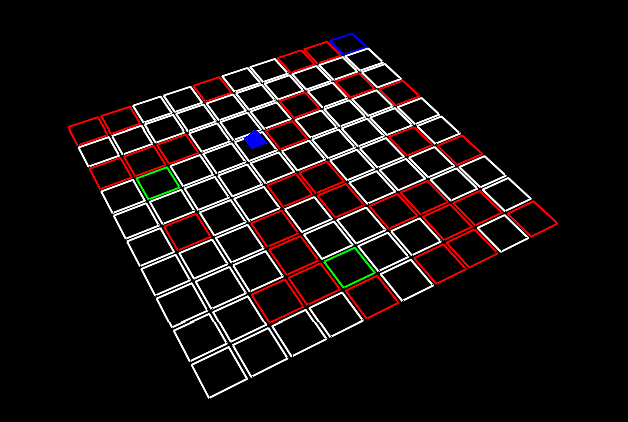
\includegraphics[scale=0.5]{example.png}
\end{frame}
\subsection{Policy}

The policy is a mapping from states to actions (or occasionally
probability distributions over actions).  This is a complete
prescription of how the agent should interact in an environment.
Finding an optimal policy will be the learning task.

\begin{frame}
	\frametitle{What is a Policy?}
	\begin{block}{Definition: Policy}
		A policy $\pi$ is a mapping from states to actions.
		\[ \pi: S \rightarrow A \]
	\end{block}
\end{frame}

\begin{frame}
	\frametitle{Value of Policy}
		The value of a policy $V^\pi(s)$ is the \textbf{total discounted
		reward} obtained by starting at a state $s$ and following the
		policy $\pi$.
		\begin{eqnarray*}	
			V^\pi(s) &=& E[R(s_0,\pi(s_0)) + \gamma (R(s_1,\pi(s_1)) + \gamma( \dots
			)) | \pi, s_0 = s]\\
			&=& E \Bigg[\sum_{t=0}^\infty \gamma^t R(s_t,\pi(s_t)) \Big| \pi, s_0 =
			s  \Bigg]
		\end{eqnarray*}	
		Here, $0 \leq \gamma \leq 1$ is the discount factor. If $\gamma =
		1$ this expectation may not exist unless the horizon is finite.
\end{frame}

\begin{frame}
	\frametitle{Alternative Value of Policy}
		The value of a policy $V^\pi(s)$ is the \textbf{long run average
		reward} obtained by starting at a state $s$ and following the
		policy $\pi$.
		\begin{eqnarray*}	
			V^\pi(s) &=& \lim_{n \to \infty} E\Bigg[\frac{\sum_{t=0}^n
			R(s_n,\pi(s_n))}{n}\Big| \pi, s_0 = s\Bigg]
		\end{eqnarray*}	
\end{frame}

\begin{frame}[allowframebreaks]
	\frametitle{Bellman Equations}
	The solution to an MDP is an optimal policy $\pi^*$ that maximizes
	$V^{\pi^*}(s)$ for all $s$:
	\[
	\pi^* = \argmax_{\pi} E\Bigg[\sum_{t=0}^\infty \gamma^t
	R(s_t,\pi(s_t))\Bigg] 
	\]
	There are $|A|^{|S|}$ policies.  For our example, that's $4^{100}
	\approx 1.6\times 10^{60}$

	\begin{block}{Recursive Bellman Equation for $\pi^*$ and $V^*$
		\footnotemark}
		\[
		\pi^*(s) = \argmax_{a\in A} R(s,a) + \gamma \sum_{s'\in S} T(s,a,s')V^*(s')
		\]
		\begin{eqnarray*}
			V^*(s) &=& R(s,\pi^*(s)) + \gamma \sum_{s' \in S}T(s,\pi^*(s),
			s') V^*(s')\\
			&=& \max_{a \in A} R(s,a) + \gamma \sum_{s' \in S}T(s,a, s') V^*(s')
		\end{eqnarray*}
	\end{block}
	\footnotetext{$V^*$ is shorthand for $V^{\pi^*}$}
\end{frame}

\section{Q-Learning}
\subsection{Learning Task}
\begin{frame}
	\frametitle{What are we learning?}
	\begin{itemize}
		\item We want to learn $\pi^*$.
			\pause
		\item We will do this by learning a $Q$ function:
			\[
			Q(s,a) = R(s,a) + \gamma \sum_{s' \in S}T(s,a, s') V^*(s')
			\]
			\pause
		\item If we learn $Q(s,a)$ then 
			\[
			\pi^*(s) = \argmax_{a\in A} Q(s,a)
			\]
	\end{itemize}
\end{frame}

\begin{frame}
	\frametitle{What are we given?}
	\begin{itemize}
		\item We are given $A$ and $S$ and a sequence 
			$\langle s_0,a_0,r_0,s_1,a_1,r_1,\dots \rangle$
			where $s \in S$ is observable and sampled by the environment
			according to $T$, $a\in A$ is chosen by the agent, and $r =
			R(s,a)$.
			\pause
		\item We are not given $T$ or $R$.
			\pause
		\item We are not going to learn $T$ or $R$.
	\end{itemize}
\end{frame}

\begin{frame}
	\frametitle{Model Free vs. Model Based Learning}
	\begin{block}{Model Free}
		The agent learns to act in specific environment, but does not
		know or learn a model of that environment.
	\end{block}
	\begin{block}{Model/Knowlege Based}
		The agent learns a model of the environment and uses the model to
		compute how to act in the environment.
	\end{block}
\end{frame}

\subsection{Q}
\begin{frame}
	\frametitle{Q Recursion}
	We can rewrite the Q function as:
	\[
	Q(s,a) = R(s,a) + \gamma E[Q(s',a)]
	\]
\end{frame}

\begin{frame}[allowframebreaks]
	\frametitle{Q Approximation and Update}
	We maintain an approximation $\hat{Q}$ of $Q$:
	\[
	\hat{Q}_{t+1}(s,a) \leftarrow \hat{Q}_t(s,a) + \alpha_t(s,a)\big[ R(s,a) + \gamma \max_{a' \in A}
	\hat{Q}_t(s',a') - \hat{Q}_t(s,a) \big]
	\]
	Where $\alpha_t(s,a)$ is the learning rate.  
	If $\alpha = 0$ than no learning occurs.  If $\alpha = 1$ than
	$\hat{Q}$ is completely overwritten at each transition.

	\pause
	This is equivalent to:
	\[
	\hat{Q}_{t+1}(s,a) \leftarrow (1-\alpha_t(s,a))\hat{Q}_{t}(s,a) + \alpha_t(s,a)\big[ R(s,a) + \gamma \max_{a' \in A}
	\hat{Q}_t(s',a') \big]
	\]

\end{frame}

\subsection{Practical Considerations}

\begin{frame}
	\frametitle{Learning Rate Schedule}
	\begin{itemize}
		\item $\alpha_t(s,a)$ must decay over time to ensure convergance.
		\item $\sum_t^{\infty} \alpha_t(s,a) = \infty$ 
	\end{itemize}
	\begin{block}{A practicle solution}
		\[
		\alpha_t(s,a) = \frac{1}{1 + visits(s,a)}
		\]
		where $visits(s,a)$ is the number of times action $a$ has been
		taken in state $s$.
	\end{block}
\end{frame}

\begin{frame}[allowframebreaks]
	\frametitle{Learning Policy: Exploration vs Exploitation}
	\begin{block}{Exploration: Random Policy}
		\begin{itemize}
			\item Choose $a \in A$ at Random in each time step.
			\item $\hat{Q}$ is guarenteed to converge to the true $Q$.
		\end{itemize}
	\end{block}
	\begin{block}{Exploitation: Locally Optimal Policy}
		\begin{itemize}
			\item Choose $a = \argmax_{a\in A} \hat{Q}(s,a)$ in each state
				$s$.
			\item $\hat{Q}$ is only guaranteed to find a local optimum.
		\end{itemize}
	\end{block}
	\begin{block}{Hybrid: Logit Quantal Response or Simulated Annealing}
		\begin{itemize}
			\item Choose $a$ according to this probability distribution:
				\[
				P(a) = \frac{e^{\beta\hat{Q}(s,a)}}{\sum_{a'\in
				A}e^{\beta\hat{Q}(s,a')}}
				\]
			\item If $\beta = 0$ this is equivalent to the random policy.
			\item As $\beta \to \infty$, this becomes the exploitative
				policy.
			\item $\beta$ may be increased over time (similar to simulated
				annealing).
		\end{itemize}
	\end{block}
\end{frame}

\section{SARSA-$\lambda$}
\subsection{Introduction}
\begin{frame}[allowframebreaks]
	\frametitle{How can we improve Q learning?}
	\begin{block}{On Policy Learning}
		Q-learning learns the Q function for the optimal policy, not the
		policy actually being followed.  Why would we want to learn a
		policy other than the optimal?
		\begin{itemize}
			\item Sometimes exploration may be ``too dangerous''.
			\item Policy may not be entirely under agent's control (e.g.
				multiagent settings).
			\item On Policy Learning allows easier application of
				eligibility traces.
		\end{itemize}
	\end{block}
	\begin{block}{Update more than one Q value at a time.}
		Q-learning only updates a single Q value at a time, so convergence
		can take a very long time if rewards are very delayed.  A clever
		method for updating multiple Q values simultaneously involves
		eligibility traces.
	\end{block}
\end{frame}

\section{Conclusions}

\subsection{Sources}
\begin{frame}[allowframebreaks]
	\frametitle{Sources}
	\nocite{*}
	\bibliography{reinforcement_learning}
	\bibliographystyle{abbrv}
\end{frame}
\end{document}

